\documentclass{article}
\usepackage{graphicx} % Required for inserting images
\usepackage[italian]{babel}
\usepackage{amsmath}
\usepackage[hidelinks]{hyperref}
\usepackage{multicol}
\usepackage{float}

\newcommand{\df}[1]{\noindent\textbf{Definizione } #1.\newline}

\title{Automazione}
\author{Leonardo Ganzaroli}
\date{}

\begin{document}

\maketitle

\addcontentsline{toc}{section}{\protect\numberline{}Introduzione}

\tableofcontents

\newpage

\hypersetup{allcolors=black}

\section*{Introduzione}

Questi appunti sono derivanti principalmente dalle dispense del corso di \textit{Automazione} che ho seguito durante la laurea Triennale di informatica all'università "La Sapienza".\newline

\noindent\textbf{N.B Alcune parti del programma non sono presenti.}

\newpage

\section{Processi industriali}

Un sistema di produzione automatizzato è composto da:
\begin{itemize}
    \item \textbf{Processo produttivo}

        Una combinazione di operazioni e trasformazioni fisico/chimiche che permettono di ottenere il prodotto finale
    
    \item \textbf{Sistema di controllo}

        Dispositivo che scambia informazioni e azioni con il processo per cambiarne il comportamento, lo fa con:
            \begin{itemize}
                \item \textbf{Sensori}
                \item \textbf{Trasduttori}
                \item \textbf{Attuatori}\newline
            \end{itemize}
    
\end{itemize}

\noindent Un impianto industriale è composto da:
\begin{itemize}
    \item Macchinari
    \item Strutture
    \item Edifici
    \item Componenti\newline
\end{itemize}

\df{Il manufacturing è l'insieme dei processi produttivi applicati alle materie prime per ottenere il prodotto finale}

\begin{figure}[ht]
    \centering
    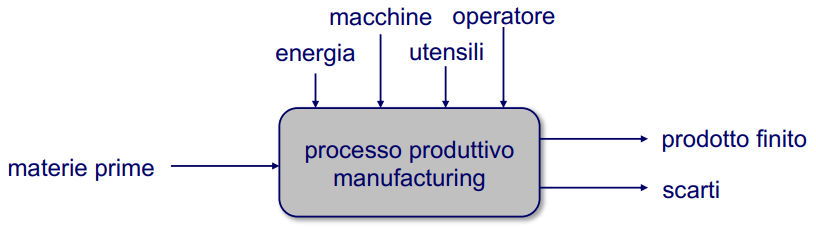
\includegraphics[width=0.75\linewidth]{manuf.png}
\end{figure}

\vspace{5pt}

\noindent Un processo produttivo è composto da una sequenza di operazioni elementari raggruppabili come:
\begin{itemize}
    \item Di lavorazione
    \item Di assemblaggio
    \item Di trasporto e stoccaggio
    \item Di test
    \item Di coordinamento e controllo
\end{itemize}

\newpage

\noindent Un'altra classificazione riguarda la gestione dell'I/O:

\begin{figure}[ht]
    \centering
    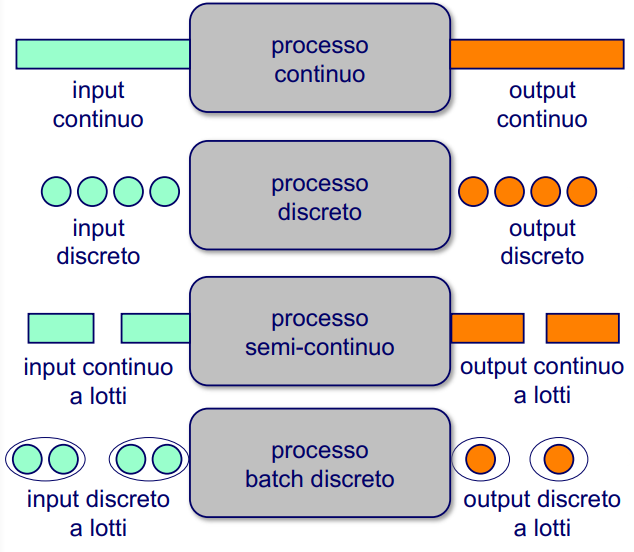
\includegraphics[width=0.7\linewidth]{proc.png}
\end{figure}

\noindent I sistemi di controllo invece possono essere:
\begin{itemize}
    \item \textbf{Logici}

        Lavorano con variabili logiche che assumono valori in un insieme numerabile (solitamente finito).
    
    \item \textbf{Diretti}

        Lavorano direttamente con i segnali.\newline
    
\end{itemize}

\subsection{Sistemi di produzione (discreti)}

I principali tipi sono:
\begin{itemize}
    \item \textbf{Linee di trasferta}
    \item \textbf{Flow Shop}
    \item \textbf{Job Shop}
    \item \textbf{Celle di produzione}
    \item \textbf{FMS}
\end{itemize}

\newpage

\subsubsection{Linee di trasferta}

\begin{itemize}
    \item Insieme di macchine/stazioni connesse in linea da un sistema di trasporto
    \item Sequenza prefissata di lavorazioni
    \item Flusso continuo di singoli pezzi
    \item Linee sincrone o asincrone\newline
\end{itemize}

\noindent La legge di Little si può applicare a linee deterministiche e mono-prodotto:
$$WIP=\text{Throughput}\times\text{Tempo di attraversamento}$$

\noindent (In regime stazionario)\newline

\noindent Per dimensionare opportunamente una linea di trasferta si segue questo procedimento:
\begin{itemize}
    \item Data un linea con $N$ stazioni, ognuna con il suo carico $C_i$ (tempo necessario)
\end{itemize}
\begin{enumerate}
    \item Il tasso di produzione è dato dalla stazione con il carico massimo
    \item Il carico massimo teorico ($CMT$) è dato dal prodotto richiesto nel periodo
    \item Si crea un grafo delle precedenze delle lavorazioni
    \item Si trova un'assegnazione ammissibile delle lavorazioni alle stazioni tale che:
        \begin{itemize}
            \item I vincoli di precedenza del grafo siano rispettati
            \item Il numero di stazioni venga minimizzato
            \item $\forall\ i\in[1,N]\ \ C_i\leq CMT$\newline
        \end{itemize}

        Per fare ciò si usa l'euristica RPWT:
            \begin{enumerate}
                \item Per ogni lavorazione si crea l'insieme $S_i$ delle lavorazioni ad essa successive
                \item Per ogni lavorazione si calcola il peso $PW_i=T_i+\sum_{k\in S_i} T_k$
                \item Si ordina per peso decrescente
                \item Fino ad esaurimento si assegna la lavorazione con peso maggiore alla prima stazione disponibile
            \end{enumerate}
        
\end{enumerate}

\noindent\rule{\textwidth}{0.5pt}

\noindent Esempio:\newline

\noindent Una linea di assemblaggio di computer richiede 14 lavorazioni e si vogliono 300 computer ogni 7 ore.

\newpage

\begin{figure}[ht]
    \centering
    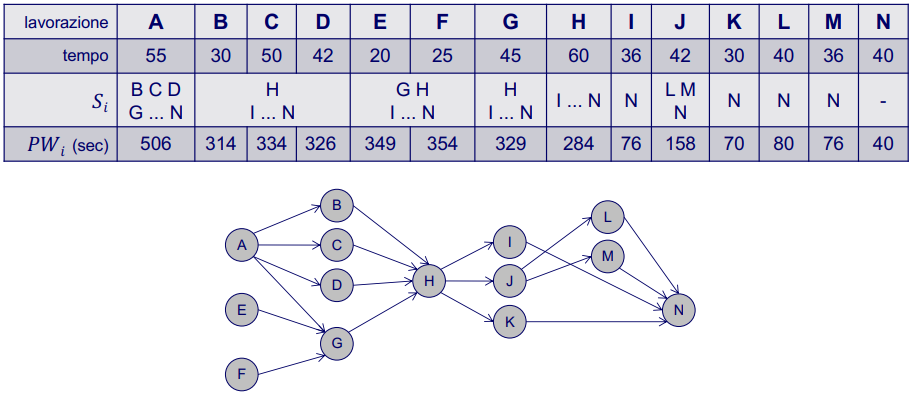
\includegraphics[width=1\linewidth]{dim.png}
    \caption{Costi e grafo}
\end{figure}

\begin{itemize}
    \item $CMT=(\frac{300}{7*3600})^{-1}=84\ [s/\text{pezzo}]$
    \item $T_{TOT}=551\ s$
    \item Macchine minime $=\frac{551}{84}\approx 7$\newline
\end{itemize}

\begin{figure}[ht]
    \centering
    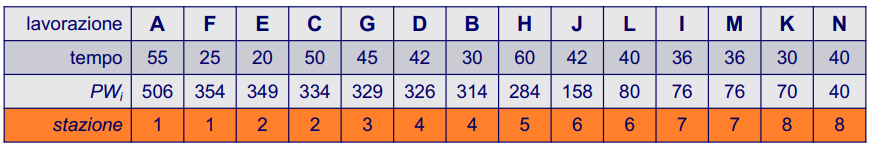
\includegraphics[width=\linewidth]{ass.png}
    \caption{Assegnamenti}
\end{figure}

\noindent Sommando il tempo mancante ad ogni stazione per raggiungere il $CMT$ e dividendolo per il numero di stazioni si ottiene lo sbilanciamento medio:
$$\frac{111}{8}=13.875\ s=16.5\%$$

\noindent\rule{\textwidth}{0.5pt}

\newpage

\subsubsection{Flow Shop}

\begin{itemize}
    \item Stazioni/macchine disposte in linea
    \item Più prodotti ma stesse lavorazioni
    \item Una macchina esegue una lavorazione\newline
\end{itemize}

\noindent In questo caso è importante minimizzare il tempo totale di completamento, nel caso di 2 macchine si segue la regola di Johnson per ogni macchina:
\begin{itemize}
    \item $t_{i1},t_{i2}$ sono i tempi di lavorazione del prodotto $i$ sulle macchine 1 e 2
\end{itemize}
\begin{enumerate}
    \item Si crea l'insieme 1 con i jobs $t_{i1}\leq t_{i2}$
    \item Si crea l'insieme 2 con i jobs $t_{i1}>t_{i2}$
    \item Si eseguono quelli nel primo in ordine crescente
    \item Si eseguono quelli nel secondo in ordine decrescente
\end{enumerate}

\noindent\rule{\textwidth}{0.5pt}

\noindent Esempio:\newline


\begin{table}[ht]
    \centering
    \begin{tabular}{c|c|c|c|c|c|c}
        Job$\setminus$Prodotti & A & B & C & D & E & $T_{TOT}$\\
        \hline
        $t_{i1}$ & 5 & 3 & 8 & 10 & 7 & 33\\
        \hline
        $t_{i2}$ & 2 & 6 & 4 & 7 & 12 & 31\\
    \end{tabular}
\end{table}

\begin{itemize}
    \item $S_1=\{B,E\}$
    \item $S_2=\{A,C,D\}$
    \item Sequenza $B,E,D,C,A$\newline
\end{itemize}

\begin{figure}[ht]
    \centering
    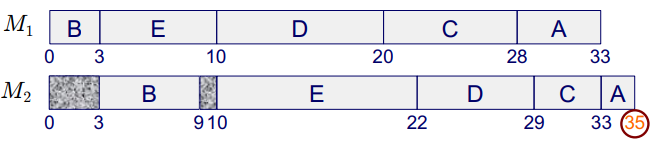
\includegraphics[width=0.65\linewidth]{gant.png}
    \caption{Diagrammi di Gantt delle macchine}
\end{figure}

\begin{itemize}
    \item $T_{MAX}=35$
    \item $t_{idle,1}=0$
    \item $t_{idle,2}=4$
\end{itemize}

\noindent\rule{\textwidth}{0.5pt}

\newpage

\noindent Si può generalizzare con 3 macchine se $max(t_{i2})\leq min(t_{i1})\vee max(t_{i2})\leq min(t_{i3})$, si creano 2 macchine equivalenti con durate $\tau_{i1}=t_{i1}+t_{i2},\ \tau_{i2}=t_{i2}+t_{i3}$ e si procede come visto, alla fine la sequenza ottenuta si applicherà con le macchine originali.\newline

\subsubsection{Altri tipi}

Job Shop:
\begin{itemize}
    \item Prodotti diversi con lavorazioni diverse
    \item Divisione in reparti
    \item Routing tra i reparti\newline
\end{itemize}

\noindent Produzione per celle:
\begin{itemize}
    \item Famiglie di prodotti con lavorazioni abbastanza omogenee
    \item Raggruppamento di gruppi di macchine in celle
    \item Flussi più semplici\newline
\end{itemize}

\noindent FSM:
\begin{itemize}
    \item Simile al precedente
    \item Uso di trasporto automatico
    \item Uso di calcolatori per il controllo del processo\newline
\end{itemize}

\begin{figure}[ht]
    \centering
    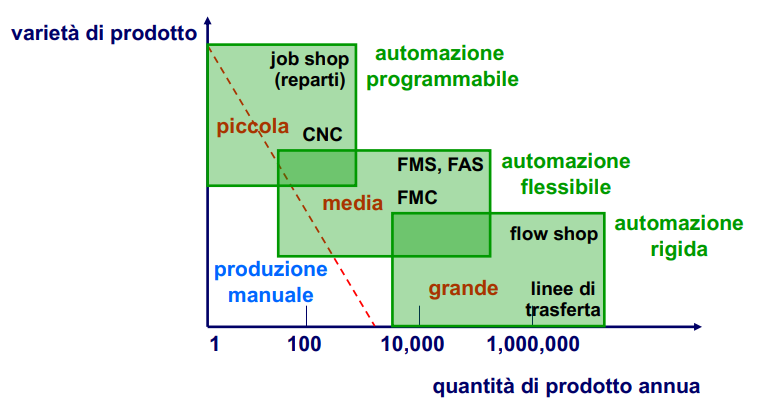
\includegraphics[width=0.8\linewidth]{prod.png}
\end{figure}

\newpage

\subsection{CIM}

\df{Il sistema di supporto alla produzione è l'insieme di attività di gestione delle informazioni riguardanti la produzione}

\df{L'Enterprise Resource Planning è un insieme di applicazioni informatiche volte all'automazione di attività amministrative, logistiche, $\ldots$ }

\df{Il Decision Support System è un software che fornisce delle funzionalità atte a migliorare il processo decisionale}

\df{Il Computer Aided Design è un insieme di software che assistono i progettisti nelle attività di progettazione}

\df{Il Computer Aided Engineering è un software per la verifica delle funzionalità del progetto}

\df{Il Computer Aided Manufacturing è un software che permette di automatizzare le prove di fattibilità del processo produttivo}

\df{Il Computer Aided Process Planning è un software che permette di automatizzare la pianificazione della produzione}

\df{Il Computer Integrated Manufacturing è un modello teorico di un sistema produttivo che integra i processi produttivi con i sistemi di automazione e i sistemi informativi gestionali}

\begin{figure}[ht]
    \centering
    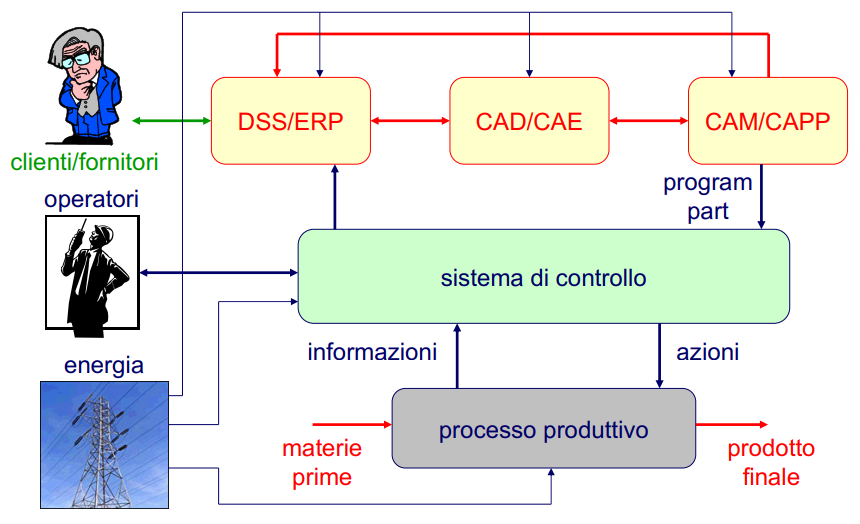
\includegraphics[width=1\linewidth]{cim.png}
\end{figure}

\subsubsection{Livelli}

\begin{figure}[ht]
    \centering
    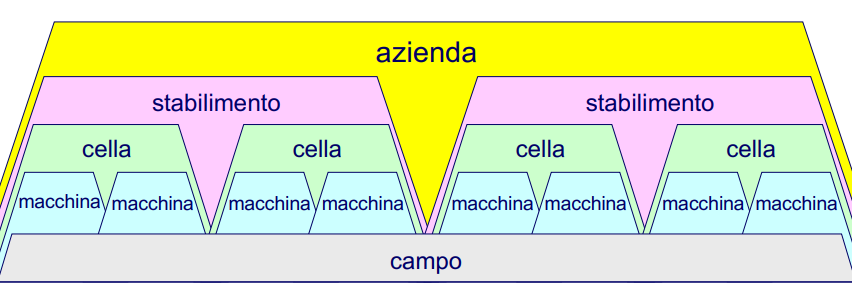
\includegraphics[width=1\linewidth]{cim2.png}
    \caption{Gerarchia CIM}
\end{figure}

\begin{itemize}
    \item \textbf{Campo}

        Contiene i componenti hardware che eseguono le attività produttive ed il loro controllo.

    \item \textbf{Macchina}

        Raggruppa gli elementi del livello precedente in gruppi atti a svolgere una certa funzionalità.

    \item \textbf{Cella}

        Raggruppa gli elementi del livello precedente in celle.

    \item \textbf{Stabilimento}

        Racchiude tutte le celle e le linee produttive facenti parte di un impianto industriale.

    \item \textbf{Azienda}

        Qui avvengono i processi gestionali di supporto ai livelli inferiori.\newline
    
\end{itemize}

\subsubsection{Reti di comunicazione}

Ad ogni livello della piramide :
\begin{itemize}
    \item Si acquisiscono informazioni
    \item Si elaborano strategie
    \item Si attuano azioni correttive
\end{itemize}

\noindent Diventa quindi di vitale importanza il sistema di comunicazione.

\newpage

\begin{figure}[ht]
    \centering
    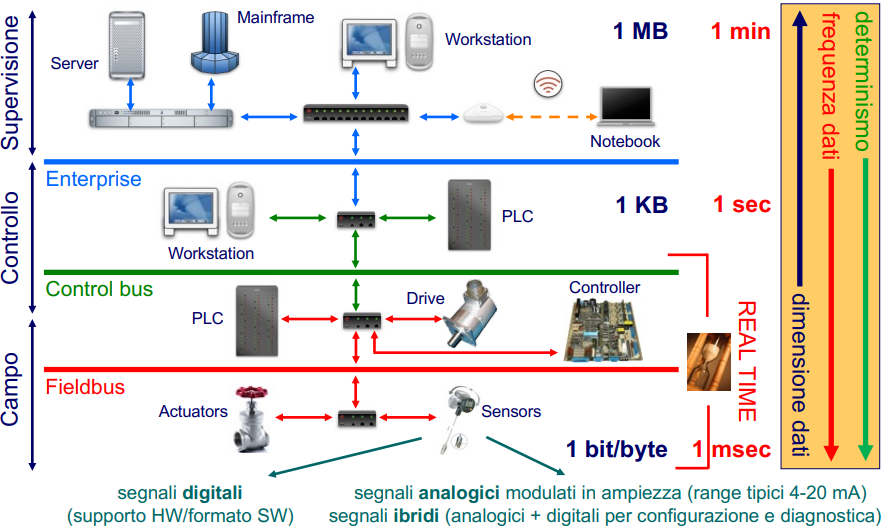
\includegraphics[width=1\linewidth]{reti.png}
\end{figure}

\begin{itemize}
    \item \textbf{Supervisione}
        \begin{itemize}
            \item Informazioni gestionali
            \item Client e Server standard
            \item Non Real-time
            \item Ethernet
        \end{itemize}
    \item \textbf{Controllo/Campo}

            \item Client e Server non standard    
            \item Dati piccoli ma frequenti
            \item Vincoli Real-time
            \item Serve determinismo
            \item Serve robustezza\newline

\end{itemize}

\noindent Usare il modello ISO-OSI risulterebbe troppo oneroso, quindi si usa il modello \textit{Fieldbus} che presenta solamente i livelli:
\begin{enumerate}
    \item Fisico
    \item Data Link
    \item Applicazione
\end{enumerate}

\section{Attuazione e controllo del moto}

Gli azionamenti elettrici sono dispositivi che convertono in modo controllato l'energia elettrica in meccanica, sono formati da 3 componenti:
\begin{enumerate}
    \item Amplificatore/Convertitore di potenza
    \item Motore elettrico
    \item Controllore\newline
\end{enumerate}

\noindent I motori elettrici hanno 2 schemi realizzativi:

\begin{figure}[ht]
    \centering
    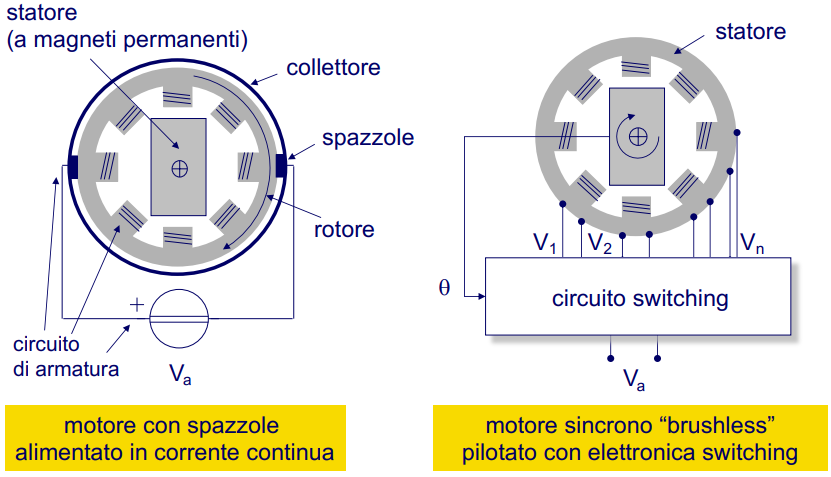
\includegraphics[width=0.7\linewidth]{mot.png}
\end{figure}

\noindent In particolare quelli a corrente continua si possono rappresentare con il seguente modello:

\begin{figure}[ht]
    \centering
    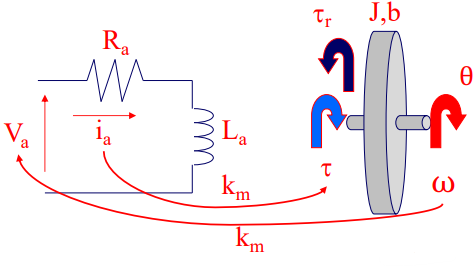
\includegraphics[width=0.7\linewidth]{dc.png}
\end{figure}

\begin{itemize}
    \item \textbf{Modello elettrico} $L_a\frac{d\ i_a}{d\ t}=V_a-R_ai_a-k_m\omega$
    \item \textbf{Modello meccanico} $J\frac{d\ \omega}{d\ t}=k_mi_a-b\omega-\tau_r$, $\ \frac{d\ \theta}{d\ t}=\omega$
\end{itemize}

\section{Sistemi di controllo Real-time}

Un sistema di controllo può definirsi Real-time sse:
\begin{itemize}
    \item Può elaborare le informazioni in modo da dare risposte logicamente corrette
    \item Può elaborare le informazioni in modo da dare risposte temporalmente corrette\newline    
\end{itemize}

\df{Il Quality of Service esprime la capacità del sistema di rispettare entrambi i vincoli di correttezza logica e temporale}

\df{Un sistema è Hard Real-time se rispetta \textbf{SEMPRE} i vincoli di correttezza}

\begin{figure}[ht]
    \centering
    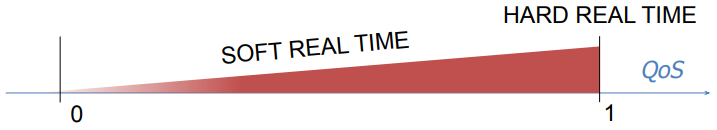
\includegraphics[width=0.9\linewidth]{qos.png}
\end{figure}

\vspace{5pt}

\df{Un task è un'unita atomica di lavoro}

\begin{figure}[ht]
    \centering
    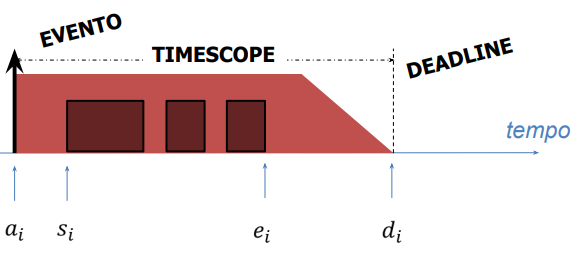
\includegraphics[width=0.7\linewidth]{task.png}
    \caption{Task $A_i$}
\end{figure}

\noindent Parametri caratteristici:
\begin{multicols}{2}
\begin{itemize}
    \item $a_i$, istante di attivazione
    \item $s_i$, istante di prima esecuzione
    \item $e_i$, istante di fine esecuzione
    \item $d_i$, deadline assoluta
    \item $C_i=e_i-s_i$
    \item $D_i=d_i-a_i$
    \item $R_i=e_i-a_i$
    \item $L_i=e_i-d_i$
\end{itemize}
\end{multicols}

\subsection{Scheduling}

\df{Un insieme di task è schedulabile se esiste un algoritmo di scheduling che permetta di rispettare tutti i vincoli}

\noindent Classificazione degli algoritmi di scheduling:
\begin{itemize}
    \item \textbf{Guaranteed} se rispetta sempre i vincoli temporali, \textbf{Best effort} altrimenti
    \item \textbf{Preemptive} se può interrompere l'esecuzione di un task in favore di un altro con priorità maggiore, \textbf{Non preemptive} altrimenti
    \item \textbf{Offline} se lo scheduling è noto a priori, \textbf{Online} altrimenti
    \item \textbf{Statico} se il dispatching dipende da parametri immutabili, \textbf{Dinamico} altrimenti\newline
\end{itemize}

\noindent Nel caso dell'automazione ha senso considerare dei task attivati periodicamente, si parla quindi di istanze dei task.\newline

\df{Il tempo di attivazione $T_i(k)$ dell'istanza $k$ di $A_i$ è l'intervallo di tempo tra l'attivazione dell'istanza $k$ e l'attivazione di $k+1$}

\df{Un task è detto periodico se il tempo di attivazione resta costante}

\noindent\textbf{Definizione} Il fattore di utilizzazione è pari a:
$$\sum_{i=1}^n\frac{C_i}{T_i}$$

\noindent Se è maggiore di 1 non esiste uno scheduling.\newline

\noindent\rule{\textwidth}{0.5pt}

\noindent Esempio:\newline

\begin{itemize}
    \item $A_1$,$T_1=8\ t.u.$, $C_1=2\ t.u.$
    \item $A_2$,$T_2=12\ t.u.$, $C_2=8\ t.u.$
    \item Fattore = $\frac{2}{8}+\frac{8}{12}\approx0.917$, potenzialmente schedulabile
\end{itemize}

\noindent\rule{\textwidth}{0.5pt}\newline

\df{Il limite superiore minimo del fattore di utilizzazione di un algoritmo di scheduling è il minimo tra i fattori calcolati per ogni possibile insieme di task periodici}

\subsubsection{Algoritmi}

In presenza di soli task periodici:
\begin{itemize}
    \item \textbf{RMPO}

        Assegna ad ogni task una priorità inversamente proporzionale al periodo di attivazione, schedulabilità garantita fino ad un fattore di $69.3\%$.

    \item \textbf{EDF}

        Assegna ad ogni task una priorità inversamente proporzionale alla sua deadline assoluta, in caso di parità si guarda il numero d'istanza minore. Schedulabilità possibile fino ad un fattore $\leq1$.

    \item \textbf{DMPO}

        Assegna la priorità in modo inversamente proporzionale a $D_i$, schedulabilità possibile solo con fattore $\leq n(2^{0.5}-1)$.
        
    \item \textbf{TS}

        Divisione del tempo in \textit{slices}, assegnazione arbitraria.\newline
    
\end{itemize}

\noindent In caso siano presenti anche task aperiodici:
\begin{itemize}
    \item \textbf{Servizio in background}

        I task aperiodici vengono eseguiti negli istanti liberi.

    \item \textbf{Server}

        Si inserisce un task periodico detto Server, i task aperiodici vengono eseguiti quando esso è in esecuzione.

    \item \textbf{Polling Server}

        Variante del precedente in cui il tempo di computazione dell'istanza dipende dai task in attesa.

    \item \textbf{Deferrable Server}

        Ulteriore variante in cui il tempo di computazione è sempre al massimo.\newline
    
\end{itemize}

\newpage

\subsection{Implementazione}

Oggigiorno qualsiasi sistema di controllo è implementato via software, per disaccopiarlo dall'hardware si usa uno strato di astrazione detto \textit{HAL}, esso si occupa dei task non real-time in modo best effort. Quelli real-time vengono gestiti tramite lo scheduler ed è presente un timer per il controllo delle deadline.\newline

\begin{figure}[ht]
    \centering
    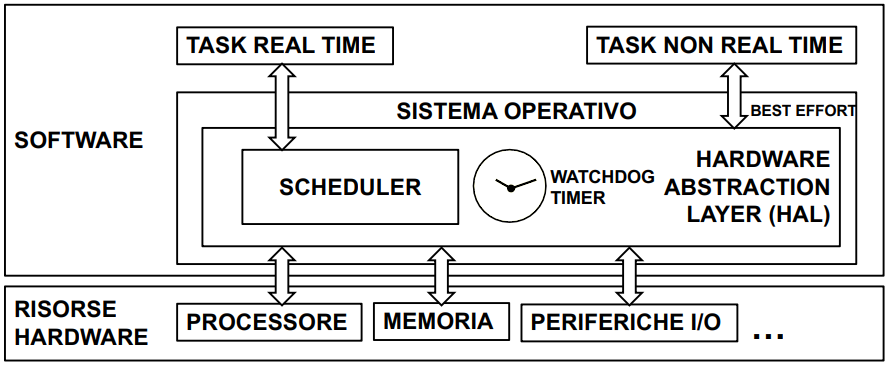
\includegraphics[width=0.75\linewidth]{hal.png}
\end{figure}

\df{Un s.o. è detto Event Driven se può schedulare un task nello stesso istante che viene attivato}

\noindent Un approccio puramente Event Driven non è realizzabile se l'unità di elaborazione è digitale, in questo caso si fa una rilevazione periodica. A livello implementativo questo metodo è migliore.\newline

\noindent In base al tipo di caratteristiche richieste i sistemi di controllo possono essere implementati in diversi modi:
\begin{itemize}
    \item \textbf{SCADA}
    \item \textbf{DCS}
    \item \textbf{Sistemi embedded}
    
    \item \textbf{PLC} e \textbf{SoftPLC}
\end{itemize}

\newpage

\section{Linguaggi per PLC}

Secondo normativa esistono 5 linguaggi per i PLC:
\begin{itemize}
    \item Grafici
\end{itemize}
\begin{enumerate}
    \item \textbf{SFC} (quello approfondito)
    \item \textbf{FBD}
    \item \textbf{LD}
\end{enumerate}
\begin{itemize}
    \item Testuali
\end{itemize}
\begin{enumerate}
    \item \textbf{ST}
    \item \textbf{IL}\newline
\end{enumerate}

\subsection{SFC}

\begin{figure}[ht]
    \centering
    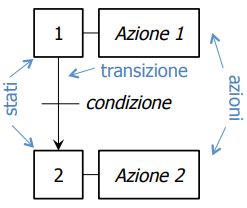
\includegraphics[width=0.5\linewidth]{sfc.png}
    \caption{Diagramma SFC}
\end{figure}

\noindent Il passaggio da uno stato al successivo può avvenire sse:
\begin{itemize}
    \item La condizione è verificata
    \item Lo stato precedente è attivo
\end{itemize}

\noindent Questo fa diventare lo stato successivo attivo e interrompe quello precedente.\newline

\noindent Ogni stato ha 2 variabili associate:
\begin{enumerate}
    \item \textbf{Marker}, indica se lo stato è attivo (nome-stato.X)
    \item \textbf{Timer}, indica da quanto tempo è attivo (nome-stato.T)\newline
\end{enumerate}

\noindent All'avvio del PLC tutti i timer vengono azzerati e solamente i marker degli stati iniziali sono posti ad 1.

\newpage

\noindent Ogni stato ha associata un'azione, essa ha la forma:
\begin{itemize}
    \item $A_m$, identificatore dell'azione

        Semplici:
            \begin{itemize}
                \item $N$, azione ripetuta ciclicamente finché lo stato è attivo
                \item $P$, azione eseguita una volta finché lo stato è attivo
                \item $S$, ripete l'azione finché non incontra $R$ in uno stato successivo
                \item $R$
                \item $L$, come $N$ o fino al tempo fornito
                \item $D$, come $N$ ma dopo un tempo di delay
            \end{itemize}

        Composti:
            \begin{itemize}
                \item $SD$
                \item $DS$
                \item $SL$
            \end{itemize}
        
    \item $Q_m$, qualificatore che definisce il tipo d'azione
    \item $V_m$, variabile che indica se l'azione è finita
\end{itemize}

\subsubsection{Strutture di collegamento}


Nel caso ci siano sequenze diverse in base a diverse condizioni si usa la divergenza:
\begin{figure}[ht]
    \centering
    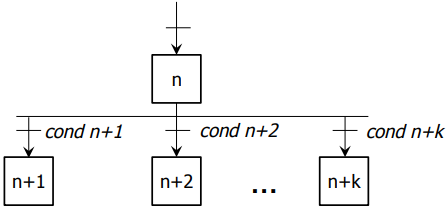
\includegraphics[width=0.7\linewidth]{div.png}
\end{figure}

\vspace{5pt}

\noindent Questa struttura deve soddisfare il vincolo della mutua esclusione per funzionare correttamente, ad ogni condizione viene aggiunto implicitamente il NAND di tutte le altre condizioni:

$$cond(n+1)=cond(n+1)*\prod_{j=1}^{k-1}!cond(n+i-j)\ \text{ con } i\in[1,k-1]$$

\newpage

\noindent Quando si usa una divergenza bisogna sempre ritornare ad un'unica sequenza, per fare ciò si usa la convergenza:
\begin{figure}[ht]
    \centering
    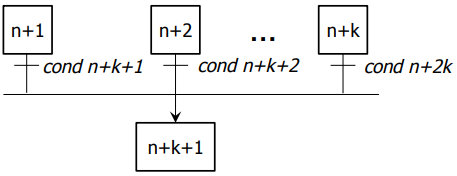
\includegraphics[width=0.7\linewidth]{conv.png}
\end{figure}

\vspace{10pt}

\noindent Se invece c'è necessità di svolgere sequenze di azioni parallele si usa il parallelismo:
\begin{figure}[ht]
    \centering
    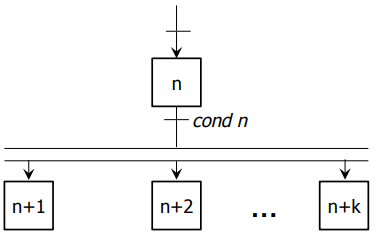
\includegraphics[width=0.6\linewidth]{par.png}
\end{figure}

\vspace{10pt}

\noindent L'equivalente della convergenza in questo caso è la sincronizzazione:
\begin{figure}[ht]
    \centering
    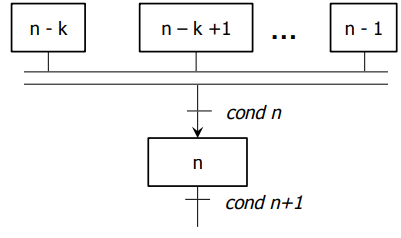
\includegraphics[width=0.6\linewidth]{sinc.png}
\end{figure}

\noindent\textbf{N.B. questa struttura "scatta" quando tutti gli stati a monte sono attivi e si verifica la condizione, in caso di necessità si possono inserire stati di attesa.}

\newpage

\noindent In presenza di risorse condivise si può usare un semaforo (uno stato) per garantire la mutua esclusione:

\begin{figure}[ht]
    \centering
    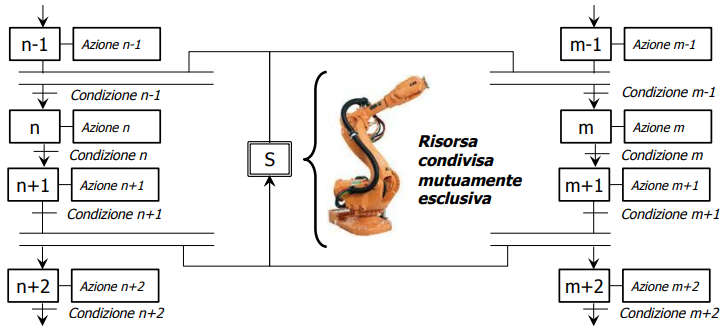
\includegraphics[width=\linewidth]{sem.png}
\end{figure}

\vspace{10pt}

\noindent Si può anche usare per sincronizzare le sequenze parallele:

\begin{figure}[ht]
    \centering
    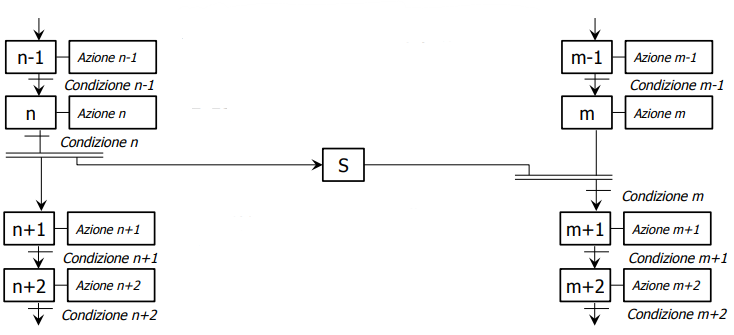
\includegraphics[width=\linewidth]{sem2.png}
\end{figure}

\vspace{10pt}

\noindent Generalmente viene impostato come stato stato iniziale per indicare che all'avvio la risorsa è disponibile.

\section{DEDS}

\textbf{Definizione} Un sistema è un insieme di componenti cooperanti ed interagenti che realizzano una funzionalità complessiva, si distinguono:
\begin{itemize}
    \item Guidati dal tempo
    \item Guidati dagli eventi\newline
\end{itemize}

\df{Un sistema dinamico ad eventi discreti evolve in base agli eventi ed ha uno spazio degli stati discreto}

\noindent Per rappresentare questi sistemi si usano diversi modelli formali:
\begin{itemize}
    \item Operazionali
        \begin{itemize}
            \item Automi
            \item Reti di Petri
            \item SFC
        \end{itemize}
    \item Dichiarativi
        \begin{itemize}
            \item Basati su equazioni
            \item Basati su regole\newline
        \end{itemize}
\end{itemize}

\subsection{Reti di Petri}

\textbf{Definizione} Un grafo di Petri è un grafo orientato e bipartito $(P,T,A,w)$ in cui:
\begin{itemize}
    \item $P$ è l'insieme dei posti (nodi)
    \item $T$ è l'insieme delle transizioni
    \item $A\subseteq(T\times P)\cup(P\times T)$ (archi)
    \item $w:A\rightarrow\mathbf{N}\setminus\{0\}$
\end{itemize}

\noindent Per esprimere la topologia si usano 2 matrici $|P|\times|T|$:
\begin{enumerate}
    \item $I$ contiene i pesi degli archi posti-transizioni
    \item $O$ contiene i pesi degli archi transizioni-posti\newline
\end{enumerate}

\begin{figure}[ht]
    \centering
    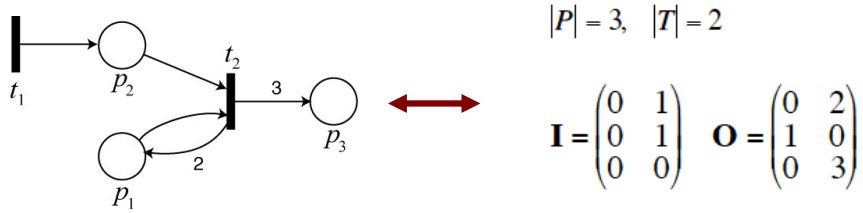
\includegraphics[width=0.9\linewidth]{pet.png}
    \caption{Esempio}
\end{figure}

\df{Una rete di Petri è un grafo di Petri con una funzione di marcatura che associa ad ogni posto un numero di token $x:P\rightarrow\mathbf{N}$}

\noindent Per rappresentare lo stato della rete si usa il vettore di marcatura con $|P|$ elementi, nel caso visto sopra potrebbe essere:
\[\begin{pmatrix}
    0\\1\\1
\end{pmatrix}\subseteq\mathbf{N^3}\]\newline

\noindent Una transizione $t_j$ è abilitata se:
$$\forall\ p_i\in I(t_j)\ \ x(p_i)\geq w(p_i,t_j)$$
\noindent Se è abilitata allora può "scattare", questo comporta un cambiamento dello stato rappresentabile con la funzione $\mathbf{N}^{|P|}\times T\rightarrow\mathbf{N}^{|P|}$.\newline

\begin{figure}[ht]
    \centering
    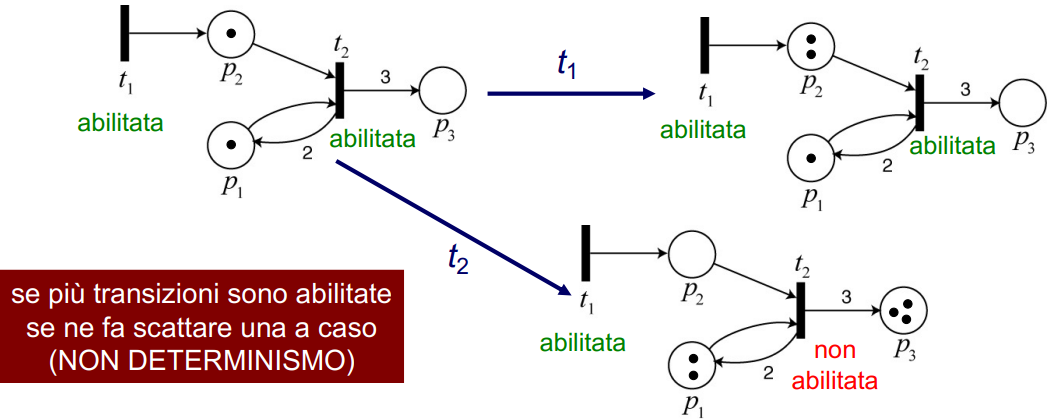
\includegraphics[width=1\linewidth]{stat.png}
    \caption{Esempio}
\end{figure}

\df{La matrice di incidenza è $C=O-I$, rappresenta l'andamento della rete}

\noindent\textbf{Definizione} Una sequenza di scatti $S$ è una sequenza di transizioni tali che:
\begin{itemize}
    \item La prima è abilitata nella marcatura corrente
    \item Ogni scatto porta ad una marcatura in cui è abilitata la transizione successiva\newline
\end{itemize}

\df{Il vettore delle occorrenze di una sequenza è un vettore $|T|$ in cui l'elemento $k$ è pari al numero di occorrenze della transizione $t_k$ in $S$}

\noindent L'evoluzione della rete data una sequenza $S$ con vettore delle occorrenze $s$ è $x'=x+Cs$.

\newpage

\noindent Proprietà strutturali delle reti:
\begin{itemize}
    \item Una marcatura $x$ è raggiungibile dalla marcatura $y$ se esiste una sequenza di scatti che porta dalla seconda alla prima
    \item Una marcatura è detta di base se è raggiungibile da tutte le altre marcature, se è anche iniziale la rete è reversibile
    \item Una transizione $t$ è viva se per ogni marcatura ne esiste un'altra raggiungibile da essa che abilita $t$
    \item La rete è viva se tutte le sue transizioni sono vive
    \item La rete è bloccante se esiste una marcatura che non abilita alcuna transizione
    \item Un posto è $k$-limitato se in ogni marcatura raggiunge un numero di token al massimo pari a $k$, illimitato altrimenti
    \item La rete è limitata se ogni suo posto è $k$-limitato con $k$ finito, se $k=1$ è anche binaria
    \item La rete è illimitata se esiste un posto illimitato
    \item La parte conservativa della rete è un sottoinsieme di posti in cui ogni possibile evoluzione mantiene una combinazione lineare di token\newline
\end{itemize}

\noindent Tipi di transizioni:
\begin{itemize}
    \item \textbf{In conflitto}

        Uno o più posti d'ingresso in comune ma con token non sufficienti a farle scattare tutte.

    \item \textbf{In concorrenza} con successiva \textbf{sincronizzazione}

        No posti in comune, tutte abilitate e seguite da posti d'uscita che sono d'ingresso per un'altra transizione comune.

    \item \textbf{In alternativa}

        In concorrenza tra loro ma in conflitto con altre.
    
\end{itemize}

\begin{figure}[ht]
    \centering
    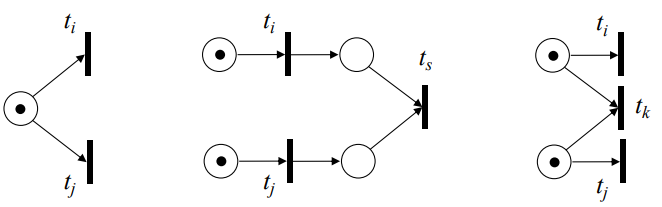
\includegraphics[width=0.6\linewidth]{trans.png}
    \caption{In ordine}
\end{figure}

\newpage

\noindent Classi di reti:
\begin{itemize}
    \item \textbf{SM}
        \begin{itemize}
            \item Ogni transizione ha un solo posto d'ingresso ed un solo posto d'uscita
            \item Numero di token fisso
            \item Viva sse esiste almeno un token ed il grafo è fortemente connesso
            \item Presenta solo conflitti
        \end{itemize}
    \item \textbf{MG}
        \begin{itemize}
            \item Ogni transizione ha un solo posto d'ingresso ed un solo posto d'uscita
            \item Viva sse ogni ciclo ha almeno un posto marcato
            \item No conflitti
        \end{itemize}
    \item \textbf{FC}
        \begin{itemize}
            \item Concorrenza e conflitti presenti ma non si influenzano tra loro
            \item Per ogni arco p-t o il posto è l'unico d'ingresso ad essa o essa è l'unica d'uscita a quel posto 
        \end{itemize}

        Se 2 o più posti hanno una o più transizioni in comune si distinguono:
            \begin{itemize}
                \item \textbf{Estesa}

                    Hanno tutte le transizioni d'uscita in comune.
                
                \item \textbf{Asimmetrica}

                    Tutte le transizioni d'uscita di uno lo sono anche dell'altro.\newline
                
            \end{itemize}
        
\end{itemize}

\noindent Alcune estensioni delle reti sono:
\begin{itemize}
    \item Reti \textbf{temporizzate}

        Aggiunta di una struttura di clock ad ogni transizione, scatto dopo la raggiunta del relativo tempo.

    \item Reti \textbf{colorate}

        Uso di diversi token, ognuno con il suo colore.

    \item Reti \textbf{con inibitori}

        Aggiunta di archi speciali verso le transizioni, se il posto con l'arco ha almeno un token la transizione puntata non può scattare.\newline
    
\end{itemize}

\subsubsection{Analisi matriciale}

(Con R(PN) si intende l'insieme delle marcature raggiungibili dalla marcatura iniziale $x_0$)\newline

\noindent\textbf{Definizione} Un vettore colonna $\gamma$ è detto P-invariante se:
$$\forall\ x\in R(PN) \ \ \gamma^T*x=\text{ costante }\ \text{ con } \gamma\in\mathbf{N}^{|P|}\wedge \gamma\neq0$$

\noindent Si cercano tra le soluzioni del sistema lineare:
$$C^T\gamma=0\ \text{ (o }\ \gamma^TC=0^T)$$\newline

\df{Il supporto di $\gamma$ è l'insieme dei posti in esso non nulli}

\noindent Si distinguono:
\begin{itemize}
    \item \textbf{Supporto minimo} se il supporto non contiene quello di nessun'altro P-invariante
    \item \textbf{Canonico} se il MCD dei suoi elementi non nulli è 1
\end{itemize}

\begin{figure}[ht]
    \centering
    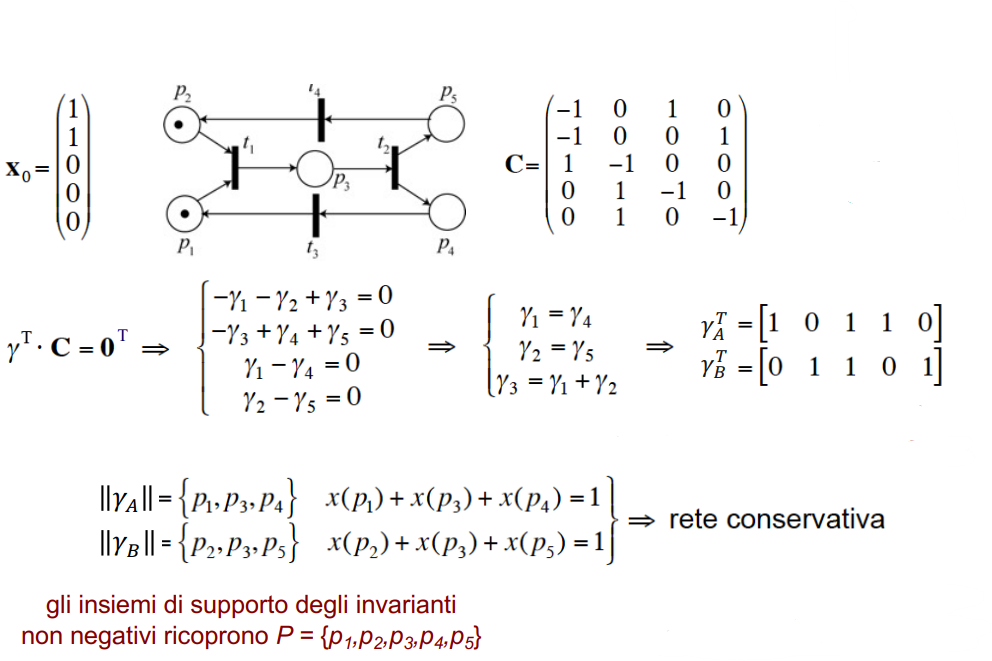
\includegraphics[width=\linewidth]{pinv.png}
    \caption{Esempio}
\end{figure}

\newpage

\noindent\textbf{Definizione} Un vettore delle occorrenze $\eta$ è detto T-invariante se:
$$x_0+C\eta=x_0$$

\noindent Si cercano tra le soluzioni del sistema lineare:
$$C\eta=0$$

\begin{figure}[ht]
    \centering
    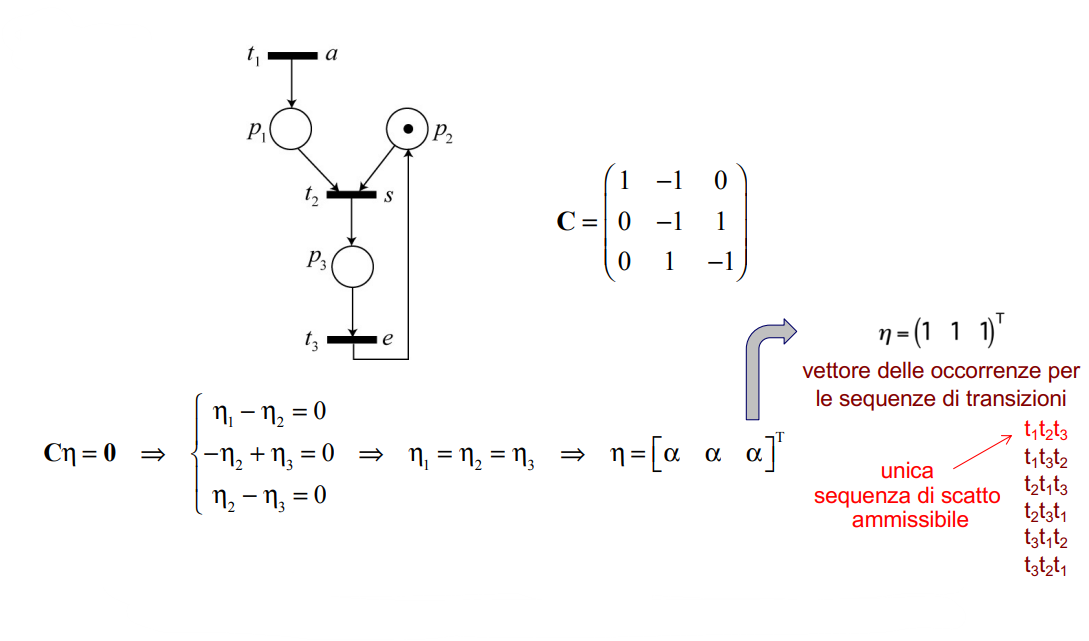
\includegraphics[width=\linewidth]{tinv.png}
    \caption{Esempio}
\end{figure}

\noindent In breve:
\begin{itemize}
    \item Un P-invariante è un insieme di posti in cui il numero di token resta costante
    \item Un T-invariante è una sequenza di scatti che partendo dalla marcatura iniziale riporta alla stessa\newline
\end{itemize}

\subsubsection{Modellazione con reti}

2 metodi:
\begin{enumerate}
    \item Fisico
        \begin{itemize}
            \item Suddivisione del sistema in sottoinsiemi elementari
            \item Modellazione degli stessi con reti elementari
            \item Composizione tra le reti ottenute
        \end{itemize}
    \item Funzionale
        \begin{itemize}
            \item Individuazione delle fasi logiche di funzionamento del sistema
            \item Identificazione delle risorse fisiche che le eseguono
            \item Allocazione delle fasi sulle risorse\newline
        \end{itemize}
\end{enumerate}

\begin{figure}[ht]
    \centering
    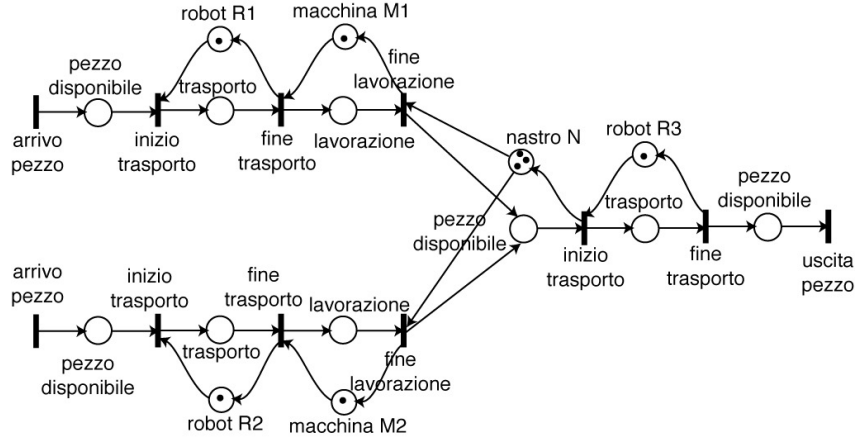
\includegraphics[width=0.9\linewidth]{es.png}
    \caption{Esempio di modellazione}
\end{figure}

\noindent Gli archi all'indietro rappresentano la disponibilità delle macchine e il numero di posti liberi sul nastro.\newline

\noindent Si può implementare una struttura di controllo nelle reti che permetta di modificare l'andamento in base alla marcatura:
\begin{itemize}
    \item \textbf{Con posti di controllo opportunamente marcati}

    Nell'esempio precedente si vogliono sul nastro 2 pezzi di $M1$ seguiti da uno di $M2$:
    \begin{figure}[H]
        \centering
        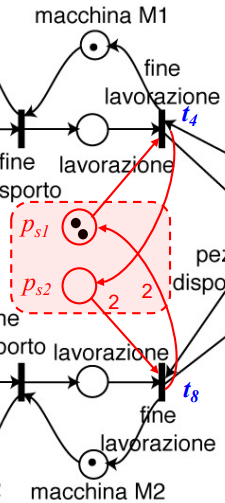
\includegraphics[width=0.19\linewidth]{contr.png}
    \end{figure}
    
    \item \textbf{Tramite invarianti e monitor}

        Si assume che il comportamento desiderato sia descrivibile con la disequazione:
        $$h^Tx\leq k\ \text{ con }h\in\mathbf{Z}^{|P|},\ k\in\mathbf{N}$$\newline

        2 casi:
        \begin{enumerate}
            \item Transizioni tutte controllabili

                Si aggiunge un posto monitor $p_i^m$ tale che:
                $$C_i^m=-h_i^TC,\ x_0(p_i^m)=k-h_i^Tx_0$$

                $C_i^m$ viene aggiunto come riga a $C$.
        
            
            \item Presenza di transizioni non controllabili

                Si usa il metodo precedente ma bisogna verificare che nessun monitor vada a disabilitare una delle transizioni non controllabili:
                $$x(p_i^m)\geq w(p_i^m,t_j)\ \text{ per ogni } t_j\text{ non controllabile}$$

                Una condizione sufficiente è che nessuna delle transizioni non controllabili abbia dei monitor in ingresso.
            
        \end{enumerate}
    
\end{itemize}

\begin{figure}[ht]
    \centering
    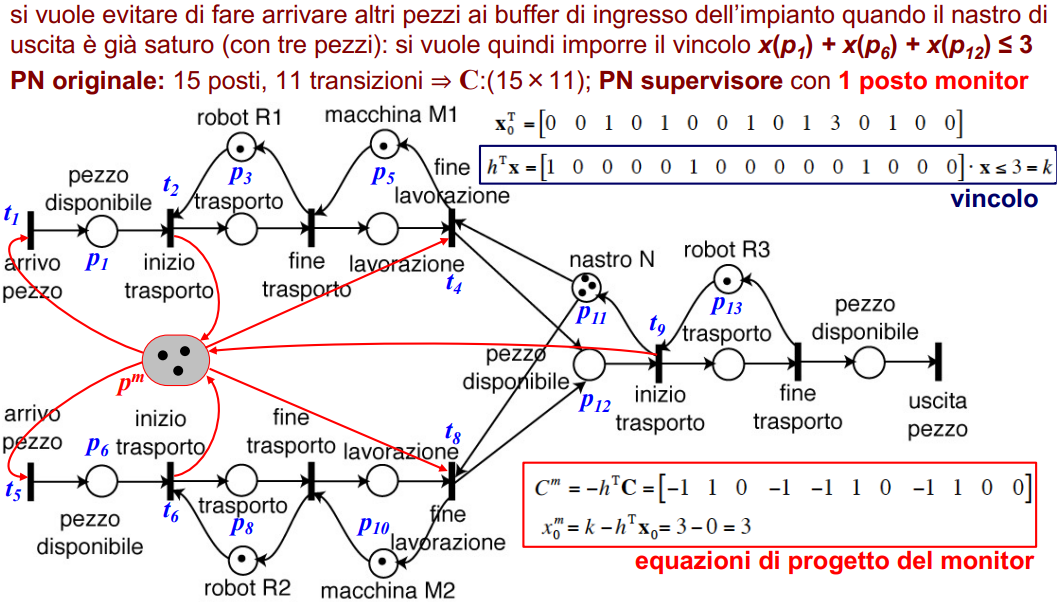
\includegraphics[width=1.1\linewidth]{mon1.png}
    \caption{Esempio primo caso}
\end{figure}

\begin{figure}[ht]
    \centering
    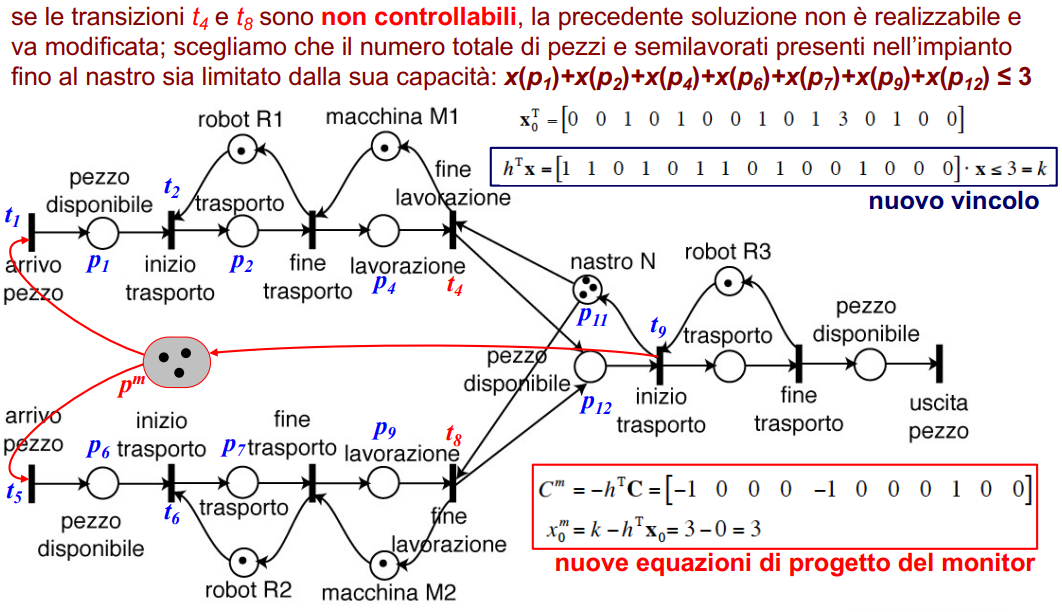
\includegraphics[width=1.1\linewidth]{mon2.png}
    \caption{Esempio secondo caso}
\end{figure}

\end{document}
